\documentclass{article}
\usepackage{tikz}
\usetikzlibrary{angles, quotes, calc}


\begin{document}
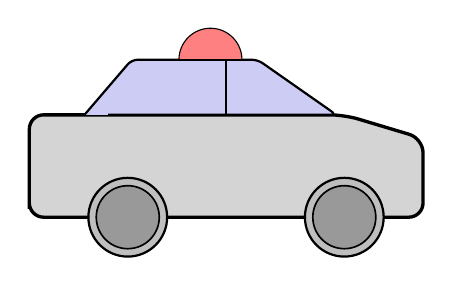
\begin{tikzpicture}
    % -- ++ means that the next point is relative to previous point
    % \shade[top color=red, bottom color=white, shading angle={135}]
    % Body
	\draw[black,fill=black!17,rounded corners=1.2ex,very thick] 
		(1.5,.5) -- ++(0,1.3) -- ++(1,0) --  ++(3,0) -- ++(1,-0.3)
			-- ++(0,-1) -- (1.5,.5) -- cycle;
	% Roof
    \draw[very thick, rounded corners=0.5ex,fill=black!20!blue!20!white,thick] 
		 (2.2,1.8) -- ++(0.6,0.7) -- ++(1.6,0) -- ++(1,-0.7) -- (2.5,1.8);
    \draw[thick]  (4,1.8) -- ++(0,0.7);
    % Wheels
    \draw[draw=black,fill=gray!50,thick] (2.75,.5) circle (.5);
    \draw[draw=black,fill=gray!50,thick] (5.5,.5) circle (.5);
    % Inner wheels
    \draw[draw=black,fill=gray!80,semithick] (2.75,.5) circle (.4);
    \draw[draw=black,fill=gray!80,semithick] (5.5,.5) circle (.4);
    % Lidar
    \draw[black, fill=red!50] (3,2.5) -- (4.2,2.5) arc(0:180:0.4) --cycle;

    % \draw[step=1.0,black,thin] (0,0) grid (7,5);
\end{tikzpicture}

\begin{figure}
	\centering
	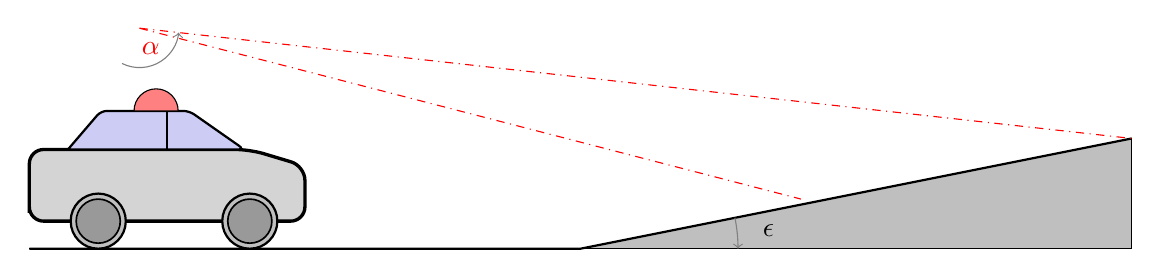
\begin{tikzpicture}[scale=0.7]
		% Define the points
		\coordinate (A) at (0,0);
		\coordinate (B) at (10,0);
		\coordinate (C) at (20,2);
		\coordinate (C2) at (14,0.9);
		\coordinate (D) at (20,0);
		\coordinate (L) at (2,4);

		\filldraw[draw=black, fill=lightgray] (B) -- (D) -- (C);

		% Draw lines between points
		\draw [thick] (A) -- (B) -- (C);
		% \draw [dotted](A) -- (L);
		\draw (A) -- (D)
		pic[draw=gray, <-, angle radius=2cm, 
		angle eccentricity=1.2, "$\epsilon$"]{angle=D--B--C};
		% Laser lines
		\draw [dashdotted, red](L) -- (C2);
		\draw [dashdotted, red](L) -- (C)
			pic[draw=gray, solid, -> , "$\alpha$"]{angle = A--L--C};
		% Angle lies at point L and starts at AL and ends at LC

        % CAR
        \coordinate (b) at ($(L) + (-2,-3.5)$);
        \coordinate (r) at ($(b) +(0.7,1.3)$);
        \coordinate (l) at ($(r) + (1.3,0.7)$);
        \coordinate (w) at ($(b) + (1.25,0)$);
        % Body
        \draw[black,fill=black!17,rounded corners=1.2ex,very thick] 
        (b) -- ++(0,1.3) -- ++(1,0) --  ++(3,0) -- ++(1,-0.3)
            -- ++(0,-1) -- (b) -- cycle;
        % Roof
        \draw[very thick, rounded corners=0.5ex,fill=black!20!blue!20!white,thick] 
            (r) -- ++(0.6,0.7) -- ++(1.6,0) -- ++(1,-0.7) -- (r);
        \draw[thick]  (r) ++(1.8,0) -- ++(0,0.7);
        % Wheels
        \draw[draw=black,fill=gray!50,thick] (w) circle (.5);
        \draw[draw=black,fill=gray!50,thick] (w) ++(2.75,0) circle (.5);
        % Inner wheels
        \draw[draw=black,fill=gray!80,semithick] (w) circle (.4);
        \draw[draw=black,fill=gray!80,semithick] (w) ++(2.75,0) circle (.4);
        Lidar
        \draw[black, fill=red!50] (l) -- ++(0.7,0) arc(0:180:0.4) --cycle;
	\end{tikzpicture}
	\caption{Tikz is hard}
\end{figure}


\end{document}